\documentclass[conference,flushend]{iaria} % Letter Size (8.5" x 11")
% The iaria class is based on IEEEtran.
% The class iaria.cls loads biblatex/biber with correct IARIA settings
% as well as a set of common packages (times, inputenc[utf8], fontenc[T1],
% graphicx, xcolor, url, orcidlink, hyperref, extdash[shortcuts])
\addbibresource{refs.bib}

\title{Trust in a Maritime Benchmark: Selection Bias, Identity Leakage, and Reproducibility in Semi-Supervised Vessel-Trajectory Classification}

\author{
  \IEEEauthorblockN{%
    Jane Smith and John Doe\,\orcidlink{0000-0002-1175-2668}}
  \IEEEauthorblockA{%
    Department of Computer Science\\
    University of …\\
    City, Country\\
    e-mail: {\tt$\lbrace$j.smith\,|\,j.doe$\rbrace$@example.org}
} }

\begin{document}
\maketitle

\begin{abstract}
Semi-supervised vessel-trajectory classification from Automatic Identification
System (AIS) data is a representative big-data analytics task: terabytes of noisy,
multi-structured maritime broadcasts are filtered, encoded, and classified. A
widely cited model, SSL-VTC, reports that adding vessel \emph{static} features
(length, width, draft) lifts four-class accuracy from 71.4\% to 92.2\%. We
reproduce the pipeline on the same public source (nationwide MarineCadastre AIS,
2019) and audit the evaluation as a data-quality and trust problem. We find three
issues. (1)~\emph{Selection bias}: the benchmark's class distribution is only
reproducible if vessels lacking complete static fields are dropped: a silent
filter driven by \emph{draft}, which is missing-not-at-random (MNAR), deleting
${\sim}92\%$ of fishing and ${\sim}66\%$ of passenger trajectories. The published
model collapses from 91.2 to 23.4 macro-F1 on the excluded vessels and scores only
64.3 on the realistic population, whereas retraining on all vessels recovers it to
88.1. (2)~\emph{Identity leakage}: the temporal split places 80.9\% of test
trajectories' vessels in training; we build a vessel-disjoint protocol and show the
static gain does \emph{not} collapse (transfers ${\sim}91\%$), a clean negative
control. (3)~\emph{Reproducibility}: the 92.2\% headline depends on an undisclosed
encoding hyperparameter, and the semi-supervised gain is marginal ($\le0.7$~pt) and
collapses at 5\% labels. We confirm the MNAR mechanism cross-region on Danish AIS,
and propose a corrected, fully-disclosed evaluation protocol; all code, configs, and
split indices are released.
\end{abstract}

\begin{IEEEkeywords}
trust in data analytics; selection bias; missing not at random; reproducibility;
semi-supervised learning; vessel trajectory classification; AIS; data quality.
\end{IEEEkeywords}

\section{Introduction}
AIS broadcasts let coastal authorities monitor vessel traffic at scale; classifying
a trajectory's \emph{vessel type} (fishing, passenger, cargo, tanker) supports
applications such as illegal-fishing detection and traffic management. SSL-VTC
\cite{duan2022sslvtc} advanced this task with a semi-supervised variational
autoencoder and, notably, the integration of \emph{static} vessel attributes
(length/width/draft) alongside kinematics (position/speed/course), reporting a large
accuracy gain.

We set out to reproduce and extend SSL-VTC and instead found that its
\emph{evaluation}, not its core idea, needs scrutiny. The static-feature claim
is broadly \emph{true} (static information is class-typical and even transfers to
unseen vessels), but three properties of the benchmark make the reported numbers
cleaner and more favorable than a realistic deployment warrants. Each property is a
data-trust failure of the kind that recurs across analytics pipelines: a silent
filtering step, leakage across a train/test boundary, and an undisclosed
preprocessing hyperparameter, echoing long-standing warnings about dataset bias
\cite{torralba2011bias}. This is a re-evaluation and reproducibility study; the
contribution is a corrected, disclosed protocol and a set of measurements that
separate genuine signal from evaluation artifacts.

\textbf{Contributions.}
(1)~We identify and quantify a \emph{static-completeness selection bias} (MNAR on
draft) and show it materially changes which vessels are evaluated and how the
published model behaves on the rest.
(2)~We provide a \emph{vessel-identity-leakage audit} with a reusable vessel-disjoint
protocol, showing the leakage is benign for the static-feature conclusion.
(3)~We document a \emph{reproducibility gap}: the headline accuracy is governed by an
undisclosed encoding hyperparameter, and the semi-supervised component is fragile.
(4)~We replicate the bias mechanism cross-region on Danish AIS and release code,
configs, split indices, and a corrected evaluation protocol.

\section{Background and Data}
\textbf{AIS and trajectories.} Ships broadcast periodic messages; each carries a
unique vessel id (MMSI). A \emph{trajectory} is a fixed-length sequence of one
vessel's messages (160 messages after the paper's extraction recipe).
\emph{Kinematic} features (LAT, LON, SOG, COG) vary over time; \emph{static}
features (LEN, WID, DRA) are constant per vessel. Following prior AIS work
\cite{nguyen2018geotracknet,nguyen2024traisformer}, each attribute is discretized
into one-hot bins and concatenated (``seven-hot'' encoding); the per-attribute
\emph{bin count} is a hyperparameter central to Section~\ref{sec:repro}. We report
accuracy and \emph{macro-F1} (mean over classes, exposing rare-class weakness) given
heavy class imbalance. The setup is four classes, a temporal split (train Jan--Apr /
val May / test Jun), a CNN with the seven-hot classifier, and an M2 semi-supervised
VAE \cite{kingma2014m2}.

\textbf{Data and reproduction.} Our source is MarineCadastre daily AIS, 2019,
Jan--Jun, U.S./Canada/Mexico coastal coverage (181 daily files, ${\sim}142$~GB
decompressed) \cite{marinecadastre}. We follow the paper's extraction (trajectory
division on $>2$\,h gaps; $\ge160$ messages; $\ge6$\,h span; abnormal-SOG removal;
sample to 160) and build two cohorts: \textbf{complete}, vessels with all of
LEN/WID/DRA, 133{,}492 trajectories; and \textbf{inclusive}, all vessels with
missing static imputed, 260{,}543 trajectories. Faithful reproduction required
matching the static seven-hot resolution (Section~\ref{sec:repro}); with fine bins
our complete-cohort model reaches 91.6\% vs the paper's 92.2\%. All numbers below are
the mean over three seeds. Fig.~\ref{fig:datasets} plots sampled trajectories by class
for both regions.

\begin{figure*}[t]
  \centering
  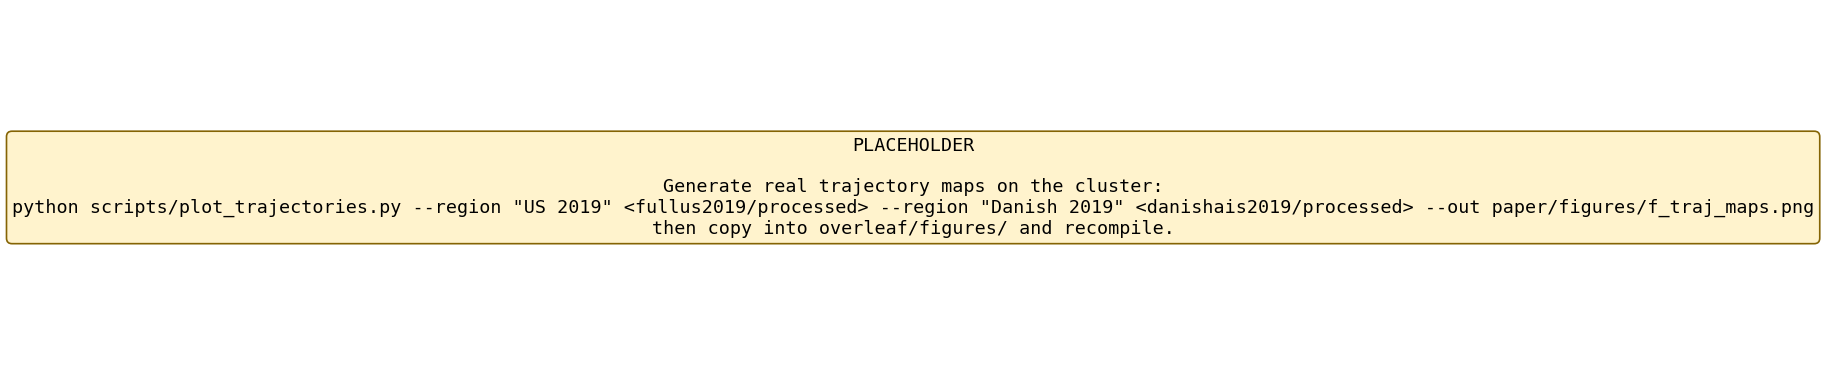
\includegraphics[width=0.92\textwidth]{figures/f_traj_maps.png}
  \caption{Sampled vessel trajectories colored by class. Left: the US MarineCadastre
  2019 cohort (US/Canada/Mexico coastal coverage). Right: the Danish Maritime Authority
  cohort (Baltic and North Sea) used for cross-region external validity. Both show the
  four target classes (cargo, tanker, passenger, fishing).}
  \label{fig:datasets}
\end{figure*}

\section{Finding 1: Static-Completeness Selection Bias}
\textbf{The benchmark's class mix is not the real ocean.} Over the full training data
(210.8\,M messages, 12{,}852 vessels) raw class shares are roughly balanced, yet the
benchmark is cargo-dominant: fishing falls from a raw 29.9\% to 2.0\% in the
benchmark, while cargo rises from 27.2\% to 53.8\%.

\textbf{Mechanism: draft is MNAR.} Length and width are widely reported; \emph{draft}
is not, and its missingness correlates with vessel type (the label), the textbook
definition of MNAR \cite{rubin1976,littlerubin2019}. Fishing vessels report draft at
12.1\% and passenger at 23.6\%, versus cargo 89.7\% and tanker 84.7\%
(Fig.~\ref{fig:draft}). Requiring all three static fields reproduces the paper's
class mix almost exactly (cargo 52.3 vs 53.8, fishing 3.6 vs 2.0), strong evidence
the benchmark applied this filter, likely inadvertently, since the method
\emph{needs} static fields.

\begin{figure}[t]
  \centering
  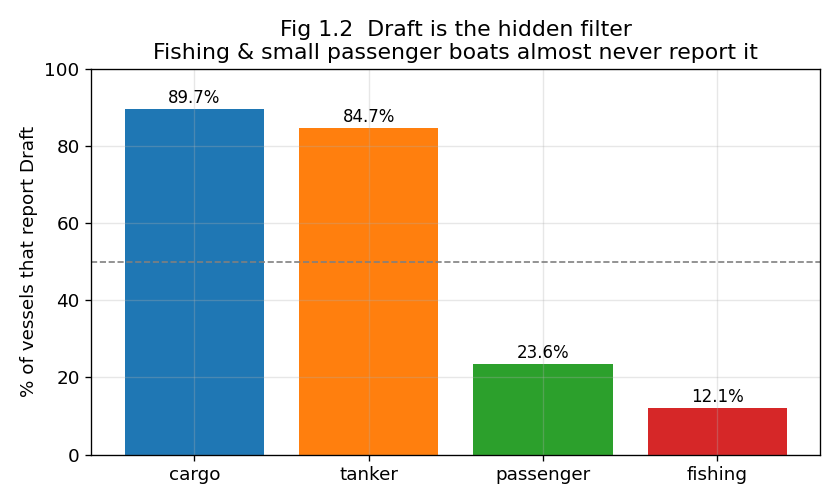
\includegraphics[width=\columnwidth]{figures/f1_2_draft.png}
  \caption{Static-field reporting rates by class. Length/width are near-universal,
  but \emph{draft} is reported by only 12.1\% of fishing and 23.6\% of passenger
  vessels versus ${\sim}85$--$90\%$ for cargo/tanker, missingness correlated with
  the label (MNAR).}
  \label{fig:draft}
\end{figure}

\textbf{The filter deletes the operational target.} Requiring complete static fields
halves the data ($260{,}543\to133{,}492$) with wildly uneven trajectory-level
survival: cargo 91.4\%, tanker 83.6\%, passenger 34.5\%, fishing 8.3\%. The benchmark
thus excludes ${\sim}92\%$ of fishing trajectories, the class central to
illegal-fishing applications.

\textbf{Consequence: the published model collapses on the excluded vessels.} We
trained the paper-strength model two ways and scored each on three populations
(macro-F1; Fig.~\ref{fig:consequence}). Model~A (trained on complete) scores 91.2 on
kept vessels but collapses to 23.4 on dropped vessels and 64.3 on the real ocean;
passenger and tanker recall fall to ${\sim}0$ because A relies on real size while
dropped vessels carry only imputed size.\footnote{A is evaluated under its own
training normalization, as in deployment; the collapse is identical under matched
normalization, ruling out a normalization artifact.} Model~B (trained on all vessels)
recovers dropped to 78.4 and scores 88.1 overall, so the failure is a protocol
artifact, not a broken method. The paper's full M2 VAE collapses identically (22.6 on
dropped), so the generative regularizer provides no robustness to the excluded
population.

\begin{figure}[t]
  \centering
  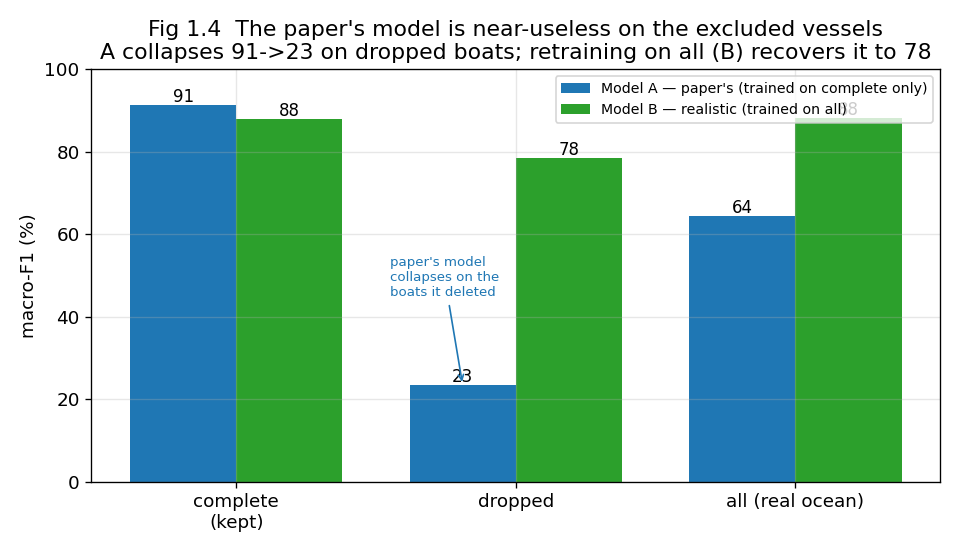
\includegraphics[width=\columnwidth]{figures/f1_4_consequence.png}
  \caption{Macro-F1 of the published-style model (A, trained on the static-complete
  slice) versus a realistic model (B, trained on all vessels) across three
  populations. A collapses on the excluded vessels (91.2$\to$23.4) and scores 64.3 on
  the real ocean; B recovers them to 88.1.}
  \label{fig:consequence}
\end{figure}

\textbf{The static benefit barely reaches the fishing target.} Per-class recall of
the realistic model, with-size vs kinematic-only (Table~\ref{tab:perclass}), shows
the size feature lifts large vessels (tanker $+22.1$, cargo $+14.5$) but barely the
fishing target ($+4.7$), which is already at 86.8\% from motion alone. The size
benefit is real but accrues to large vessels; the operational fishing class gains
little and is well-classified from kinematics.

\begin{table}[t]
  \centering
  \caption{Per-class recall (realistic model): kinematic-only vs adding static size.}
  \label{tab:perclass}
  \begin{tabular}{lccc}
    \hline
    Class & Motion only & + Size & Size boost \\
    \hline
    Fishing (target) & 86.8 & 91.5 & $+4.7$ \\
    Passenger        & 82.6 & 89.5 & $+6.9$ \\
    Cargo            & 74.4 & 88.9 & $+14.5$ \\
    Tanker           & 61.0 & 83.1 & $+22.1$ \\
    \hline
  \end{tabular}
\end{table}

\section{Finding 2: Vessel-Identity Leakage (benign)}
Static features are constant per vessel, an identity fingerprint. The temporal
split leaks identity: 80.9\% of test trajectories belong to a vessel also in training
(74.6\% vessel overlap); a vessel-disjoint split (partition MMSIs, stratified by
class) gives 0\%. We re-ran the static ablation under both protocols on a faithful
91.6\% model. The static gain (Full $-$ kinematic-only) does \emph{not} collapse: it
moves from $+18.7$ on the leaky temporal split to $+17.0$ on the vessel-disjoint
split (Fig.~\ref{fig:nocollapse}). About 91\% of the static benefit transfers to
unseen vessels, full-model accuracy drops only ${\sim}2$~pts, and fishing recall stays
high. The leakage is real but does \emph{not} inflate the static-feature result: a
rigorous negative control. A small ${\sim}9\%$ identity component appears only at fine
encoding resolution; the dominant signal is class-typical.

\begin{figure}[t]
  \centering
  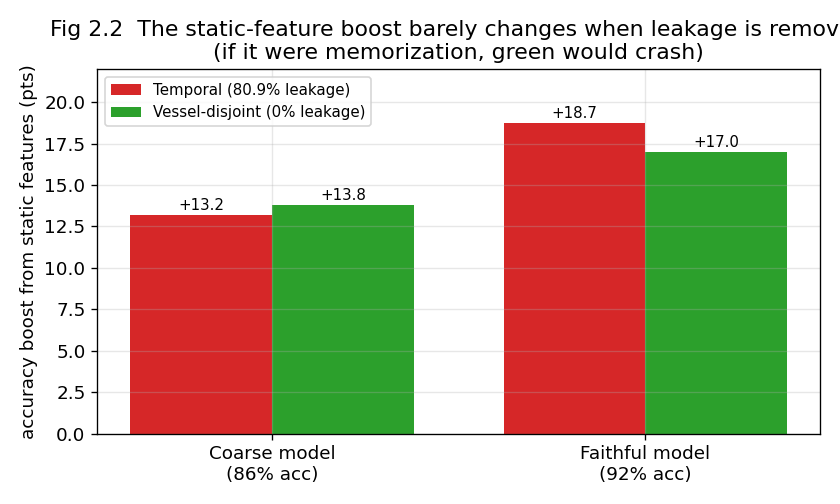
\includegraphics[width=\columnwidth]{figures/f2_2_nocollapse.png}
  \caption{Static-feature gain under the leaky temporal split versus a vessel-disjoint
  split (0\% MMSI overlap). The gain transfers (${\sim}91\%$), confirming the
  conclusion is not an artifact of identity leakage.}
  \label{fig:nocollapse}
\end{figure}

\section{Finding 3: Reproducibility}
\label{sec:repro}
\textbf{The headline rides an undisclosed hyperparameter.} We reproduced everything
from the paper yet plateaued at 86.0\% vs the reported 92.2\%. The cause is the
unspecified static seven-hot bin resolution. A controlled sweep (kinematic bins fixed)
moves Full accuracy from 86.0 (40 bins) to 88.6 (80), 90.5 (120), and 91.8 (200) with
no other change (Fig.~\ref{fig:bins}). Diagnostics rule out optimizer, scheduler, and
checkpoint selection: both cosine and constant learning-rate schedules cap at
${\sim}86$ at every epoch. The headline is therefore not reproducible from the paper
as written.

\textbf{The semi-supervised component is fragile.} Reproducing SSL-VTC against a
labeled-only baseline on faithful data, the M2 gain is marginal ($+0.7$ at 20\%
labels, $+0.2$ at 40\%, $-0.0$ at 60\%; the paper reports a clear advantage). At the
5\%-label setting the model collapses to majority-class prediction: the reconstruction
ELBO swamps the classifier at extreme label scarcity, precisely where the largest
semi-supervised benefit is claimed.

\begin{figure}[t]
  \centering
  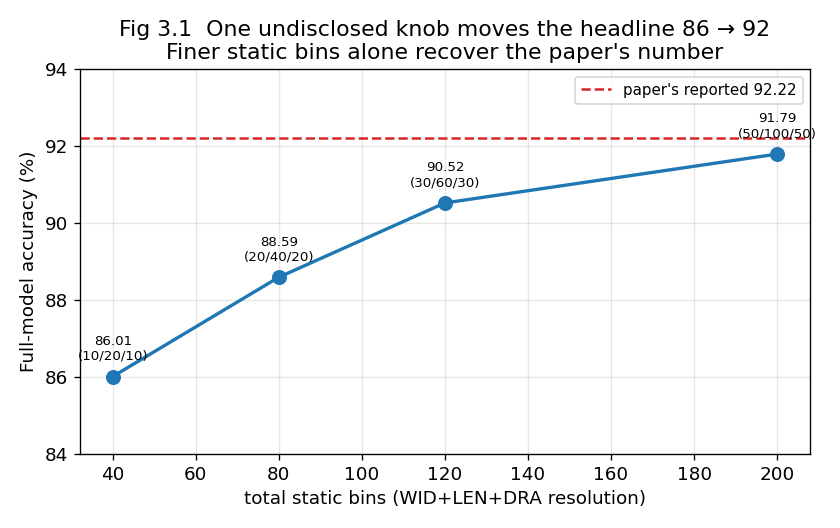
\includegraphics[width=\columnwidth]{figures/f3_1_bins.png}
  \caption{Full-model accuracy versus static seven-hot bin resolution (kinematic bins
  fixed). The undisclosed bin count alone moves accuracy 86.0$\to$91.8, closing nearly
  the entire gap to the reported 92.2\%.}
  \label{fig:bins}
\end{figure}

\section{External Validity: Danish AIS}
To test whether MNAR draft-missingness is US-specific, we replicated the mechanism
check on Danish Maritime Authority open AIS (May 2019, 2\,M messages, 1{,}464 unique
vessels; a different region, fleet mix, and regulator) \cite{dma_ais}
(Table~\ref{tab:danish}). The rank order is identical: fishing reports draft at the
lowest rate in both datasets, cargo and tanker at the highest. Absolute rates differ
(Danish fishing vessels are more professionally regulated), but the structural gap
(fishing $\ll$ cargo/tanker) is preserved. The MNAR mechanism is a property of AIS
broadly, not a US-data artifact.

\begin{table}[t]
  \centering
  \caption{Draft-reporting rate by class, US vs Danish AIS (cross-region).}
  \label{tab:danish}
  \begin{tabular}{lcc}
    \hline
    Class & US 2019 & Danish 2019 \\
    \hline
    Cargo            & 89.7\% & 97.8\% \\
    Tanker           & 84.7\% & 98.9\% \\
    Passenger        & 23.6\% & 77.6\% \\
    Fishing          & 12.1\% & 47.5\% \\
    \hline
  \end{tabular}
\end{table}

\section{A Corrected Evaluation Protocol}
We recommend: (1)~\emph{keep static-incomplete vessels} and impute missing fields
instead of deleting them (Model~B recovers the excluded population); (2)~\emph{report
per-class recall and macro-F1} so weak rare-class performance is visible; (3)~\emph{use
vessel-disjoint splits} (no MMSI in both train and test) to remove identity leakage;
(4)~\emph{disclose all preprocessing hyperparameters}, especially encoding bin
resolution, or use a learned encoder to remove the knob; (5)~\emph{evaluate on the
inclusive population by default}, reporting the static-complete subset only as a
clearly-labeled secondary slice.

\section{Limitations and Conclusion}
We cannot prove the original filter was intentional; we show it is the unique filter
reproducing the paper's distribution (cargo/tanker within ${\sim}1$~pt). Our data
vintage differs slightly (133k vs the paper's 115k trajectories) though shapes match.
Findings~1, 2, and 3.1 use the supervised CNN seven-hot classifier, exactly the
model the static tables and 92.2\% headline are reported on, while Finding~3.2 and
the VAE collapse check use the full M2 autoencoder; the corrected protocol transfers to
any model.

SSL-VTC's central idea, that static features help vessel-type classification, is
sound and even transfers to unseen vessels. But its benchmark silently selects a
static-reporting, cargo-heavy subpopulation on which the published model collapses
when deployed realistically, leaks vessel identity (though benignly), and reports a
headline that depends on an undisclosed hyperparameter. The science survives; the
evaluation needed fixing. All code, configs, split indices, and figure-generation
scripts are released to support reproduction.

\printbibliography
\end{document}
